\RequirePackage{fix-cm}
\documentclass[conf]{new-aiaa}

\usepackage[utf8]{inputenc}
\usepackage{graphicx}
\usepackage{siunitx}
\sisetup{group-separator = {,}}
\usepackage{booktabs}
\usepackage{enumitem}
\usepackage{float}
\usepackage{amsmath}
\usepackage[version=4]{mhchem}
\usepackage{longtable,tabularx}
\usepackage{placeins}
\usepackage{multirow}
\usepackage{booktabs}
\usepackage{latexsym}
\usepackage{multicol}
\usepackage{subcaption}
\usepackage{hyperref}
\usepackage[sort&compress,numbers]{natbib} % For bibtex \citet, \citep
\usepackage{hypernat} % To get natbib to play nicely with hyperref
\usepackage{doi} % For getting hyperlinked DOI in the references

%% Custom modifications of hyperlinks.
% This is not from the AIAA template standard
\usepackage{xcolor}
\colorlet{mblue}{blue!40!black}
\hypersetup{bookmarksnumbered=true,colorlinks=true,linkcolor=mblue,citecolor=mblue,urlcolor=mblue}

\setlength\LTleft{0pt} 

\hypersetup{
    pdfauthor={Peter Atma}, % insert author here
	pdftitle={Aviation 2023 Paper}, % insert title here
	pdfsubject={Comparing Hydrogen and Jet-A for an N+3 Turbofan with Water Recirculation using Gradient-Based Optimization}, % insert keywords here
}

\graphicspath{{../figures/}}

\title{Comparing Hydrogen and Jet-A for an N+3 Turbofan with Water Recirculation using Gradient-Based Optimization} % change
\author{Peter N.~Atma\footnote{MSE Student, Department of Aerospace Engineering, AIAA Student Member}}
\author{Andrew H~.R.~Lamkin\footnote{Ph.D.~Candidate, Department of Aerospace Engineering, AIAA Student Member}}
\author{Joaquim R.~R.~A.~Martins\footnote{Pauline M. Sherman Collegiate Professor, Department of Aerospace Engineering, AIAA Fellow}}
\affil{University of Michigan, Ann Arbor, MI, 48109}

\begin{document}

\maketitle

% ==================================================
%	Abstract
% ==================================================
\begin{abstract}
  Advances in commercial propulsion technology led to the development of efficient high bypass ratio turbofan engines with larger overall pressure ratios and internal temperatures.
  Current trends suggest that geared ultra high bypass ratio turbofans are the next generation of commercial propulsion systems.
  Furthermore, the emphasis on decreasing emissions has driven the exploration of hydrogen-powered aircraft, adding to the already challenging design space.
  Carrying and burning hydrogen introduces complexity and weight penalties that we must offset using the fuel's thermodynamic and chemical properties.
  In this study, we model a closed-loop water recirculation system with a zero-dimensional thermodynamic model and compare the benefits between Jet-A and hydrogen fuels.
  We perform a gradient-based optimization parameter sweep to explore the trade-offs between performance and emissions using both fuels with water recirculation.
  The results quantify the design space for next-generation propulsion concepts that can take advantage of hydrogen fuel's thermodynamic properties to reduce emissions and improve performance.
\end{abstract}

\section{Introduction}
% Message 1: Motivation to incorporate low-emission fuels and techniques
The effects of climate change are pushing the aviation industry towards hydrogen-fueled propulsion systems as a solution to reduce emissions.
N+3 technology estimates for engines that burn hydrocarbon fuels suggest that higher efficiencies can be achieved by designing ultra high bypass ratio (UHBR) turbofans with small cores and high overall pressure ratios (OPR)~\cite{Jones2017a}.
Higher OPR and smaller cores challenge the limits of compressor and turbine design, placing an upper bound on potential performance and emissions improvements.
Switching to hydrogen as the primary fuel source reduces carbon dioxide emissions immediately, but adds complexity and weight that can offset the benefits~\cite{Adler2023}.
However, hydrogen is a versatile fuel with advantageous molecular and thermodynamic properties that can be exploited to increase the performance and reduce emissions.
We introduce a closed-loop water recirculation model that demonstrates the possible efficiency gain when hydrogen is used for purposes other than combustion.

% Message 2: Background and references to support using H2 and water injection in HBTF engines
Water injection is the process of introducing water upstream of the combustor as finely atomized droplets.
NASA, Boeing, and Rolls-Royce studied this concept and suggested that this technique reduces the NOx emissions as much as 47 percent~\cite{Daggett2010}.
Additionally, water injection improves fuel efficiency and thrust output with lower combustion temperatures that can improve the lifetime of turbine blades and reduce noise~\cite{Daggett2010}.
Traditional propulsion systems that burn hydrocarbon fuels would require external demineralized water storage on the aircraft for water injection~\cite{Mourouzidis2015}.
The added weight of tanks, pumping, and ducting makes this concept infeasible for a conventional aircraft.
The main product of hydrogen combustion is water vapor~\cite{Strom2002}.
We can recover the vapor from the exhaust stream with condensers and recirculate it upstream to eliminate additional storage requirements.
If hydrogen is used as the fuel it can then be used as a heat sink for the condenser~\cite{Boggia2002}.
This system represents a closed water feedback loop inside the propulsion cycle.
Pratt and Whitney are actively researching this technology to increase the efficiency of hydrogen-powered propulsion~\cite{arpa-e_2021}.

Zero-dimensional cycle modeling is an efficient tool for predicting the initial design, performance, and emissions of new propulsion concepts.
Zero-dimensional analysis uses a first-principles approach with a chemical equilibrium analysis (CEA) thermodynamics solver~\cite{Gordon1994} that considers the molecular species of different fuels.
The industry standard for thermodynamic cycle analysis is the Numerical Propulsion System Simulation (NPSS) framework~\cite{JonesNPSS}.
NPSS is a modular object-oriented library that models engine components as individual blocks with specialized thermodynamic solvers.
\citet{Hendricks2019} created a new tool called pyCycle with the same functionality as NPSS, with the addition of analytical derivatives~\cite{Gray2017b}.
pyCycle is built on top of the OpenMDAO framework~\cite{Gray2019a} to facilitate gradient-based optimization and leverage hierarchical solver structures.

% Message 3: Introduce the extension of the HBTF and propose novel contributions
In this work, we analyze the thermodynamic benefits of a closed-loop water vapor recovery and injection system in a high-bypass turbofan engine.
We develop pyCycle components for water injection and vapor recovery to quantify the benefit of a closed loop recirculation system.
We use gradient-based optimization to minimize fuel burn subject to performance requirements using both Jet-A and hydrogen at a range of flight conditions.
The optimized results show the trade-off between complexity, performance, and efficiency for Jet-A and hydrogen fuels.
Finally, we present a design space study that demonstrates the necessary condenser technology levels for efficient water recovery.

This work is organized as follows. First, in Section~\ref{sec:method}, we introduce the turbofan model and explain the water injection and water recovery components.
In Section~\ref{sec:optprob} the implementation of the multipoint optimization problem is discussed.
Finally, we present the optimized results and discuss the condenser design space study in Section~\ref{sec:results}.

\section{Methodology}
\label{sec:method}
% Engine Architecture: Describe the flow path of the engine and establish the mechanical coupling.
The UHB turbofan model is the NASA advanced technology N+3 engine~\cite{Jones2017a}.
The N+3 reference cycle is a UHB ratio geared turbofan that could be available in the 2030 to 2040 time frame.
The flow path consists of an inlet that directs ambient air through a fan, followed by a duct that splits the flow into a core and a bypass stream, each ending in a core and bypass nozzle, respectively.
The low pressure system is split into two mechanical subsystems.
First, the fan is connected to the gearbox that reduces the shaft speed to decrease fan tip speeds.
Second, the gearbox attaches to the low-pressure shaft that connects to the low-pressure compressor (LPC) and low-pressure turbine (LPT).
The high pressure compressor (HPC) is connected to the high pressure turbine (HPT) by the high pressure shaft.
Figure~\ref{fig:N3_original} shows a simplified UHB turbofan engine flow path.
We introduce the closed-loop water recovery system as a feedback cycle that transports water from the exhaust to upstream of the compressors.
The recovery system injects vaporized water into the core stream just upstream of the HPC.
The vapor recovery component is located just upstream of the core nozzle to extract water from the exhaust and recycle it back to the injector.
Figure~\ref{fig:n3_clvr} shows the water vapor recovery loop implemented in a turbofan engine.

In this section we present the full engine layout and provide details on the multipoint zero-dimensional modeling approach.
We explain the implementation and assumptions of the water recovery model and the coupling with the thermodynamic cycle.

\begin{figure}[hbt!]
  \centering
  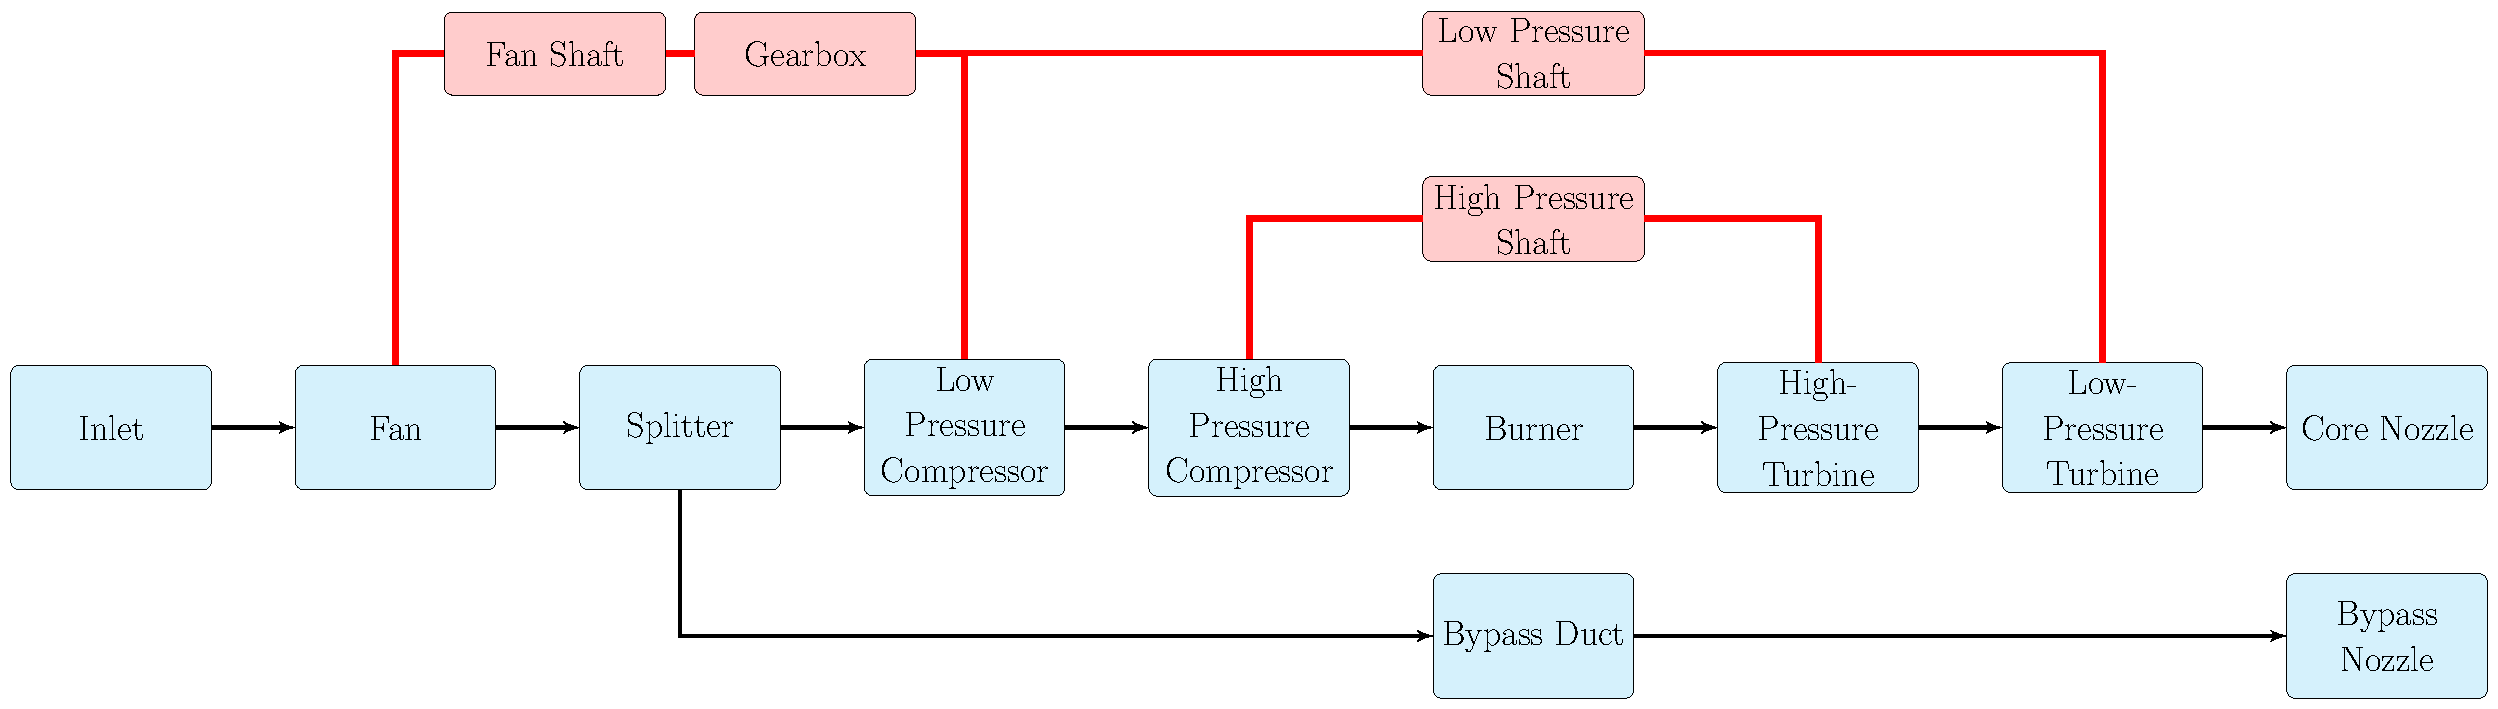
\includegraphics[width=1.0\textwidth]{N3_cycle.pdf}
  \caption{
    Simplified layout of the N+3 engine cycle, adapted from~\citet{Hendricks2019}.
    Black arrows are flow connections, red lines are mechanical connections, blue boxes are cycle elements, red boxes are shaft elements.
    Flow stations are identified with bubble text.
  }
  \label{fig:N3_original}
\end{figure}

\subsection{Water Recovery Model}
We implemented the closed-loop water recovery system as a feedback cycle that extracts water from the exhaust stream and injects it upstream of the HPC.
We chose this injection location following a study by NASA, Boeing, and Rolls-Royce~\cite{Daggett2010} that claims water injection directly into the combustor is unnecessary.
The water vapor recovery component sits downstream of the LPT and extracts water from the flow before exiting the core nozzle.
We assume that a fraction of the total water available in the exhaust stream is recovered and that there are no pressure or temperature losses associated with this process.
The component flow interface and mechanical connections, including the water injector and water extractor, are depicted in Figure~\ref{fig:n3_cycle}.

\begin{figure}[hbt!]
  \centering
  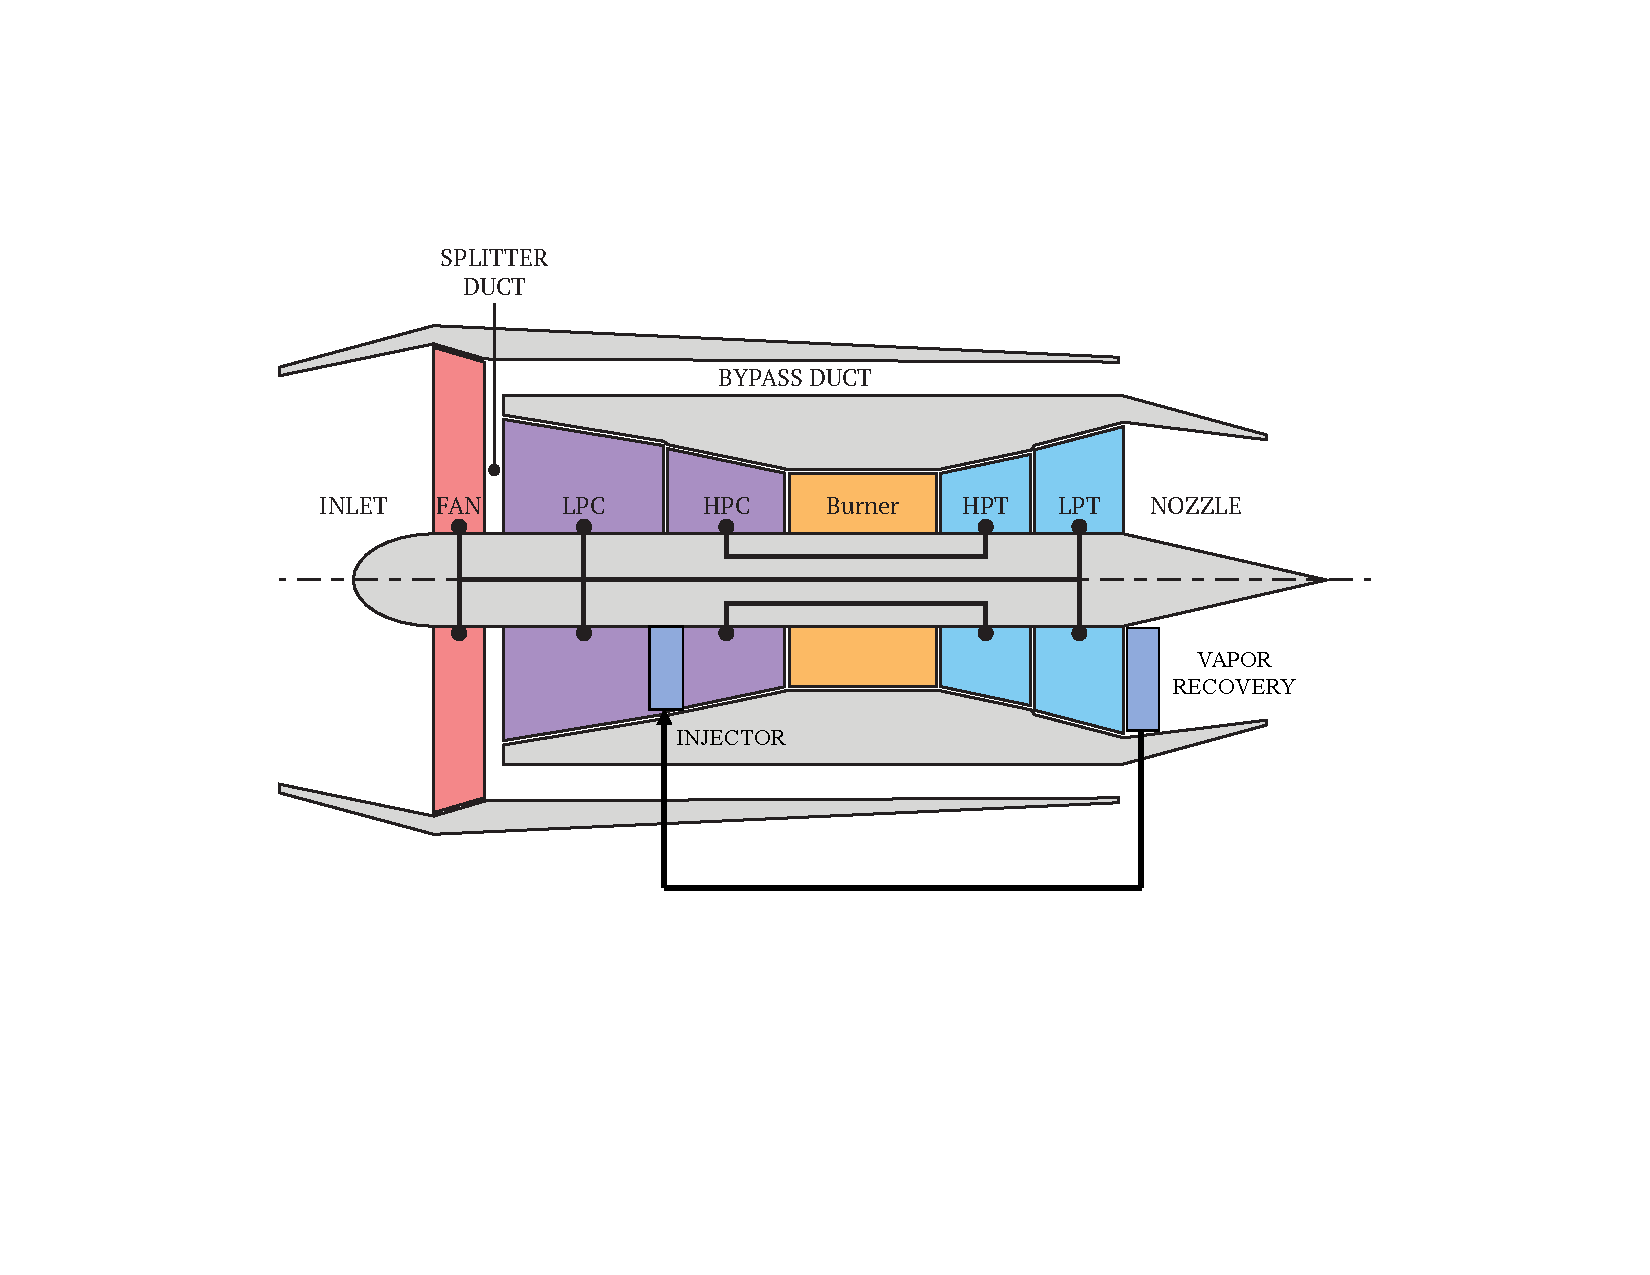
\includegraphics[width=0.75\textwidth]{turbofan_wvr.pdf}
  \caption{
    Configuration of a high-bypass turbofan model with an integrated closed-loop water vapor recovery and injection system.
    The water vapor recovery system (extractor) extracts a fraction of the water in the core stream and re-injects it upstream of the high-pressure compressor.
    This diagram illustrates the feedback effect that this implementation has on the overall core flow.}
  \label{fig:n3_cycle}
\end{figure}

To account for the humidity of the inlet air as well as the increased humidity after water injection, we modified the composition of the air mixture upstream of the combustor.
pyCycle provides a \texttt{wet-air} dataset that introduces \ce{H2O} molecules to the composition of air.
We prescribe atmospheric mass-specific humidity as a water-to-air ratio (WAR) that is defined as the ratio of \ce{H2O} to air in the reactants of the inflow mixture.
\citet{Kalnay1996} give the humidity values for each flight condition, provided in Table~\ref{tab:flight_conds}.

We introduce two thermodynamic models in pyCycle to capture the effects of water recirculation.
A water injector adds water to the flow upstream of the HPC, while a water extractor diverts a portion of the water in the flow away from the exhaust stream.
The injector operates similarly to fuel injection in the pyCycle combustor component.
We determine a WAR that is analogous to the fuel-to-air (FAR) ratio in the combustor.
This WAR is used to compute the chemical species present in the flow at the current thermodynamic state, determined by the incoming flow.
The new species composition and thermodynamic state are determined using the pyCycle CEA solver~\cite{Gray2017b}.
The water injector inputs are the mass flow rate and mass fraction of water.
We can solve for the mass flow rate on a mixture basis using the WAR, or directly by specifying the mass flow rate of water.
A schematic of the injector is shown in Figure~\ref{fig:injector} where \ce{Y_{\ce{H2O}}} is the mole fraction of water molecules.

\begin{figure}[hbt!]
  \centering
  \begin{subfigure}[t]{0.49\textwidth}
    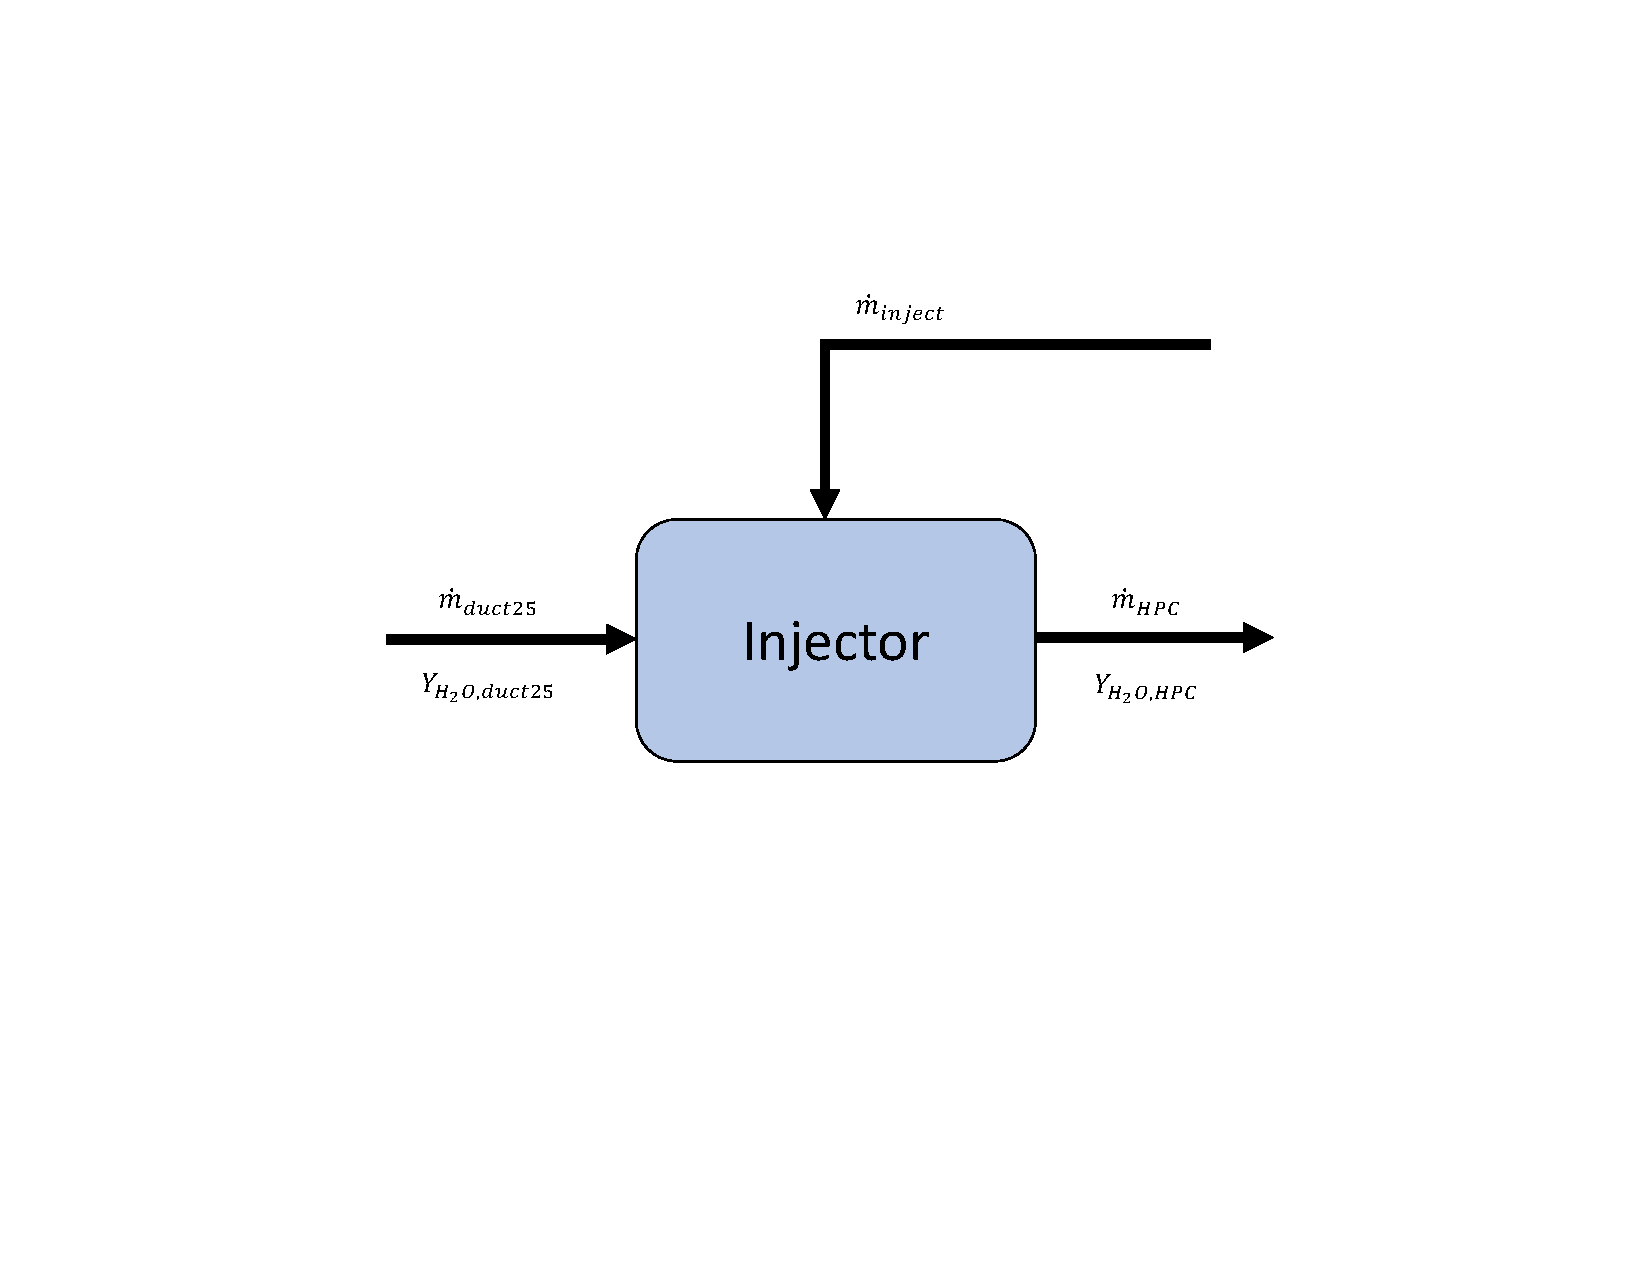
\includegraphics[width=\textwidth]{injector.pdf}
    \caption{
      Water from the extractor is simply injected into the core flow upstream of the high-pressure compressor.
    }
    \label{fig:injector}
  \end{subfigure}
  \hspace{2pt}
  \begin{subfigure}[t]{0.49\textwidth}
    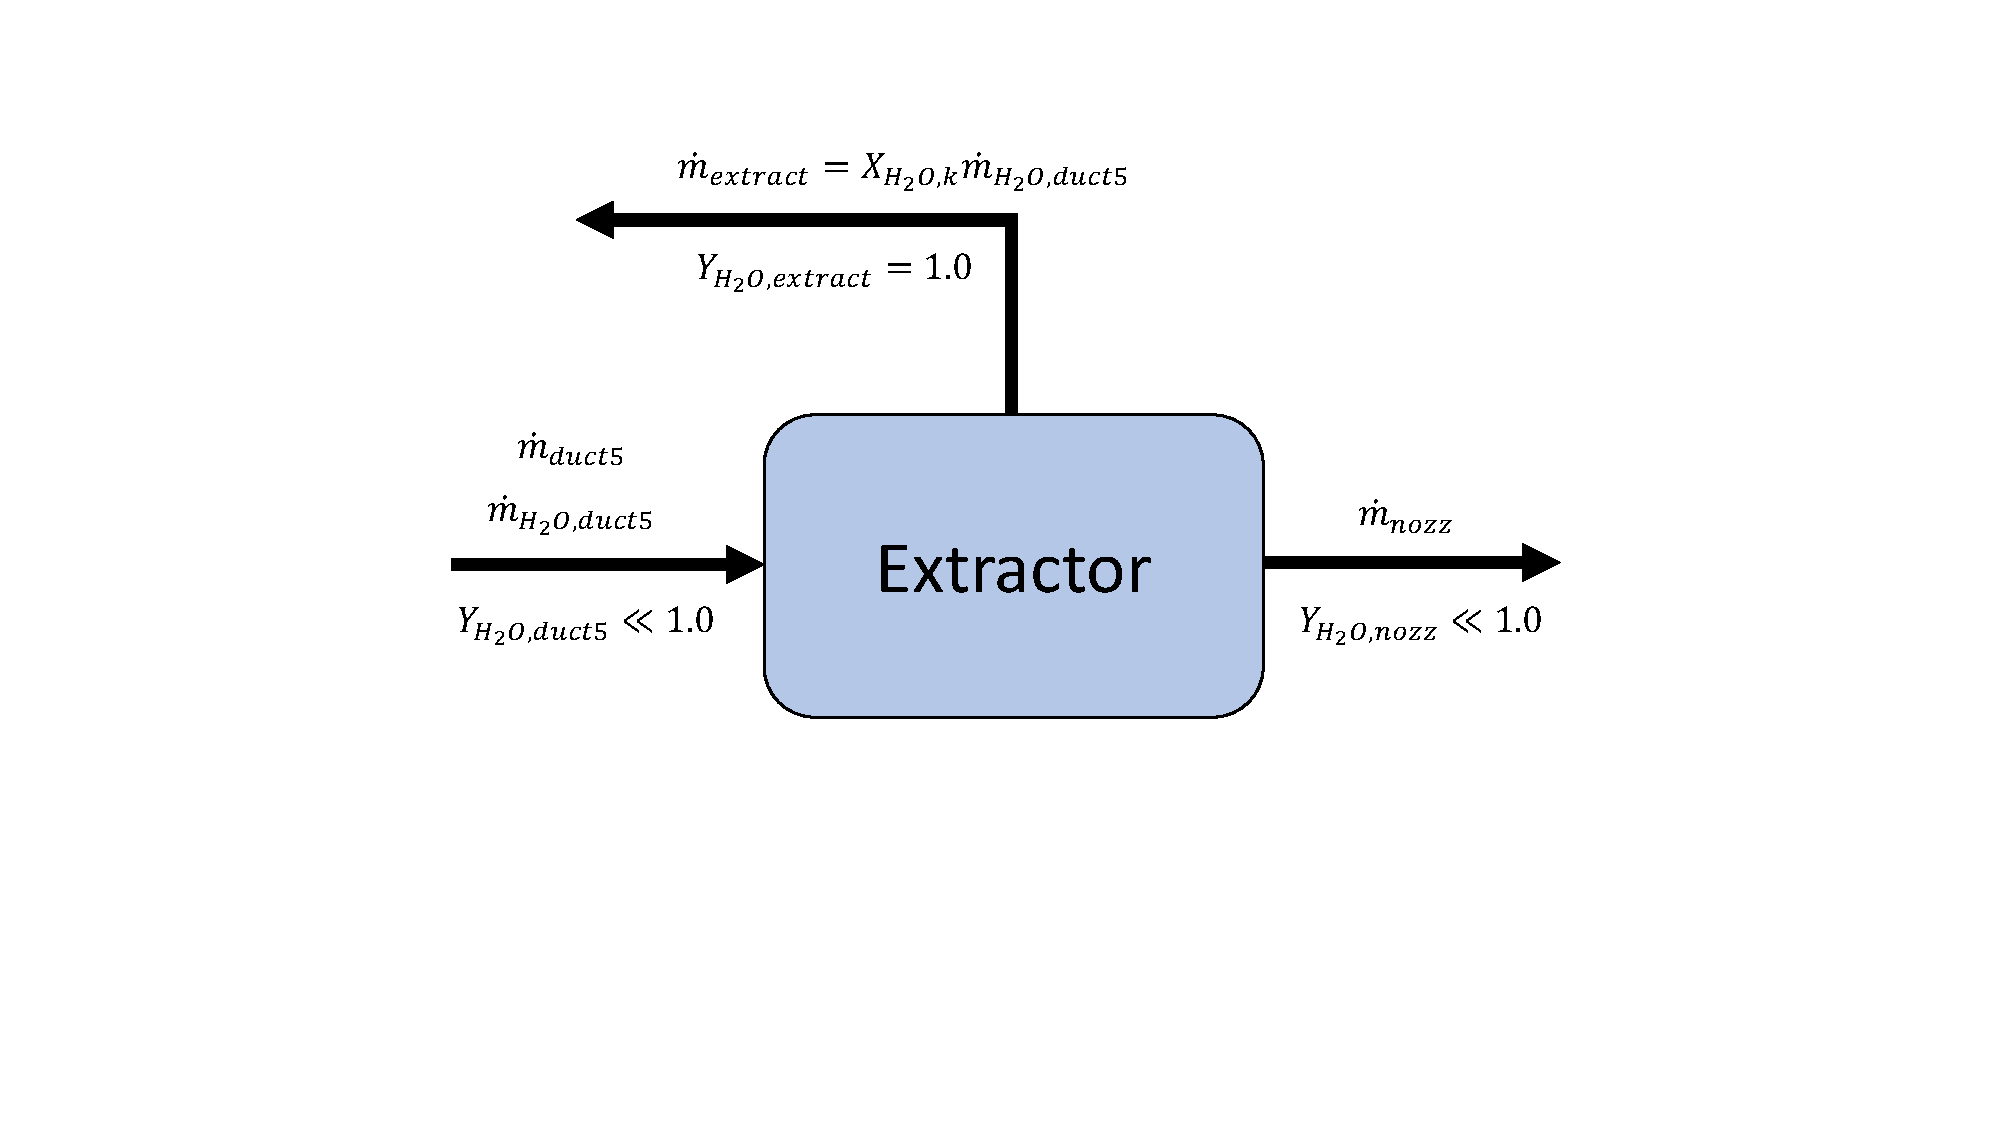
\includegraphics[width=\textwidth]{extractor.pdf}
    \caption{
      We extract a fraction of the mass flow of water determined by the molar composition.
      The extracted water is routed from Duct5 back upstream to the injector and the rest is exhausted out the nozzle.
    }
    \label{fig:extractor}
  \end{subfigure}
  \caption{Injector (left) and extractor(right) diagrams that show the inputs and output streams of each component.
    The inputs and outputs show which flow values are used to compute the amount of recirculated water.}
  \label{fig:extract_inject}
\end{figure}

The water extractor model diverts a fraction of a specific species from one flow path to another.
The CEA solver calculates the inflow composition and the extractor separates a specific species based on a mass fraction input.
The composition of the core stream is updated to represent the remaining mixture after the extractor model removes the species from the incoming flow.
We then solve for the thermodynamic state and flow path areas at the outflow of both extractor streams.
A simple schematic of the extractor is shown in Figure~\ref{fig:extractor} where \ce{Y_{\ce{H2O}}} is the mole fraction of water molecules and \ce{X_{\ce{H2O}}} is the mass fraction of water that is recovered from the core stream.
We connect one outflow stream of the extractor to the inflow stream of the injector to complete the water recirculation system.

The model results in a mismatch between the mass flow rate upstream of the HPC and the mass flow rate exiting the core nozzle.
To preserve conservation of mass, we treat the water recirculation as a nonlinear cycle that must converge before the engine calculation is physically balanced.
In this model, we are assuming the water molecules are removed from the exhaust stream with no pressure or temperature losses.
We also assume the injected water molecules are at the same pressure and temperature as the air flow just before the HPC.
We illustrate the water recirculation loop and the nonlinear solver connections in Figure~\ref{fig:N3_xdsm_full}.

\begin{figure}[hbt!]
  \centering
  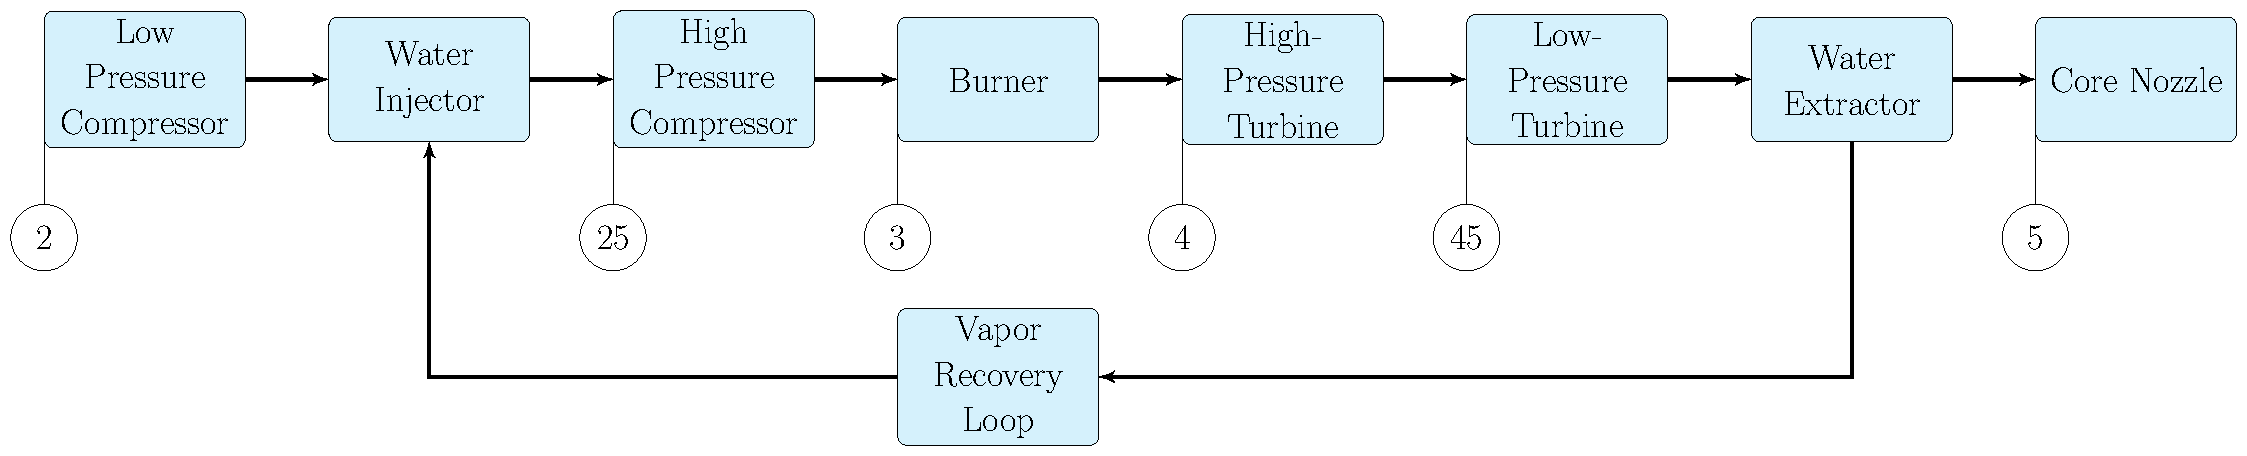
\includegraphics[width=1.0\textwidth]{N3_CLVR_cycle.pdf}
  \caption{
    Simplified layout of the N+3 engine cycle with the closed-loop vapor recovery.
    Black arrows are flow connections, blue boxes are cycle elements.
    Flow stations are identified with bubble text.
  }
  \label{fig:n3_clvr}
\end{figure}

\subsection{Multipoint Propulsion Model}
The N+3 model is a collection of components that combine to form a unified zero-dimensional cycle.
The model consists of twenty-five different elements that define the flow path and the mechanical systems.
Thermodynamic quantities are solved and exchanged using CEA at flow path boundaries represented by black arrows between blue flow path components in Figure~\ref{fig:N3_original}.
The fan, gearbox, low pressure, and high pressure systems are connected by three mechanical shafts depicted in red in Figure~\ref{fig:N3_original}.

We impose \emph{balance} equations to satisfy the physical governing equations, conservation laws, and design rules.
Balance relationships are formulated as equations in the form $r(u)=0$ where $r$ is a residual function and $u$ is an implicit state variable.
We use Newton based solvers to find the value of the state variables that drive the set of balance residuals to zero.
\citeauthor{Hendricks2019} provide the extensive set of balance equations with further details on the construction of the nonlinear system for the N+3 model.

We operate the engine cycle in different modes depending on the desired conservation relationships, design rules, and flight conditions.
In ``on-design'' mode, we prescribe cycle inputs such as turbo machinery efficiencies, pressure ratios, and combustion temperatures.
The ``off-design'' mode inherits the flow path areas and turbo machinery map scalars from the ``on-design'' analysis.
This approach is known as multi-design point (MDP)~\cite{Schutte2009} analysis.
MDP analysis simultaneously considers the performance and design requirements at each operation to automatically calculate a feasible design.

The ``on-design'' point is top-of-climb (TOC) with ``off-design'' conditions at rolling takeoff (RTO), sea-level static (SLS), and cruise (CRZ).
Table~\ref{tab:flight_conds} shows the different altitudes and mach numbers for each flight condition.

\begin{table}[hbt!]
  \centering
  \caption{Altitude and mach numbers at each of the flight conditions considered in the multipoint formulation.
    The humidity ratios were computed from humidity data~\cite{Kalnay1996}.
  }
  \begin{tabular}{l r r r r l}
    \hline
    Parameter      & TOC     & RTO   & SLS   & CRZ     & Units      \\
    \hline
    Altitude       & 35000   & 0     & 0     & 35000   & \si{ft}    \\
    Mach           & 0.8     & 0.25  & 0.0   & 0.8     & -          \\
    Humidity Ratio & 0.00017 & 0.009 & 0.009 & 0.00017 & \si{kg/kg} \\
    \hline
  \end{tabular}
  \label{tab:flight_conds}
\end{table}

The design rules at SLS ensure that the turbo machinery and flow paths meet the static thrust target.
Rolling takeoff limitations constrain the upper limit of the combustor temperature and subsequently the cooling requirements of the turbines.
The cooling mass flow rates ($\dot{m}_{\rm{cool},k}$) are passed from the RTO point to all other flight conditions creating a cyclic connection.
We add a fuel burn objective at cruise to optimize the engine performance during the longest flight segment.
We size the water recovery system at the CRZ condition because it has the greatest impact on fuel burn over the flight envelope.
Similarly to $\dot{m}_{\rm{cool},k}$, the water recovery mass flow rates ($\dot{m}_{\rm{water},k}$) are connected back to the other operating points.
Figure~\ref{fig:N3_xdsm_full} is an extended design structure matrix (XDSM)~\cite{Lambe2012a} diagram depicting the coupled multipoint model.
The interconnections between flight conditions create a nonlinear cyclic loop with feedback between flight conditions.
The converged model represents a feasible multipoint engine that accounts for design considerations and conservation laws at all four operating conditions.
We direct the reader to the N+3 multipoint model definition in the paper by \citet{Hendricks2019} for the detailed description of the balance relationships.

\begin{figure}[hbt!]
  \centering
  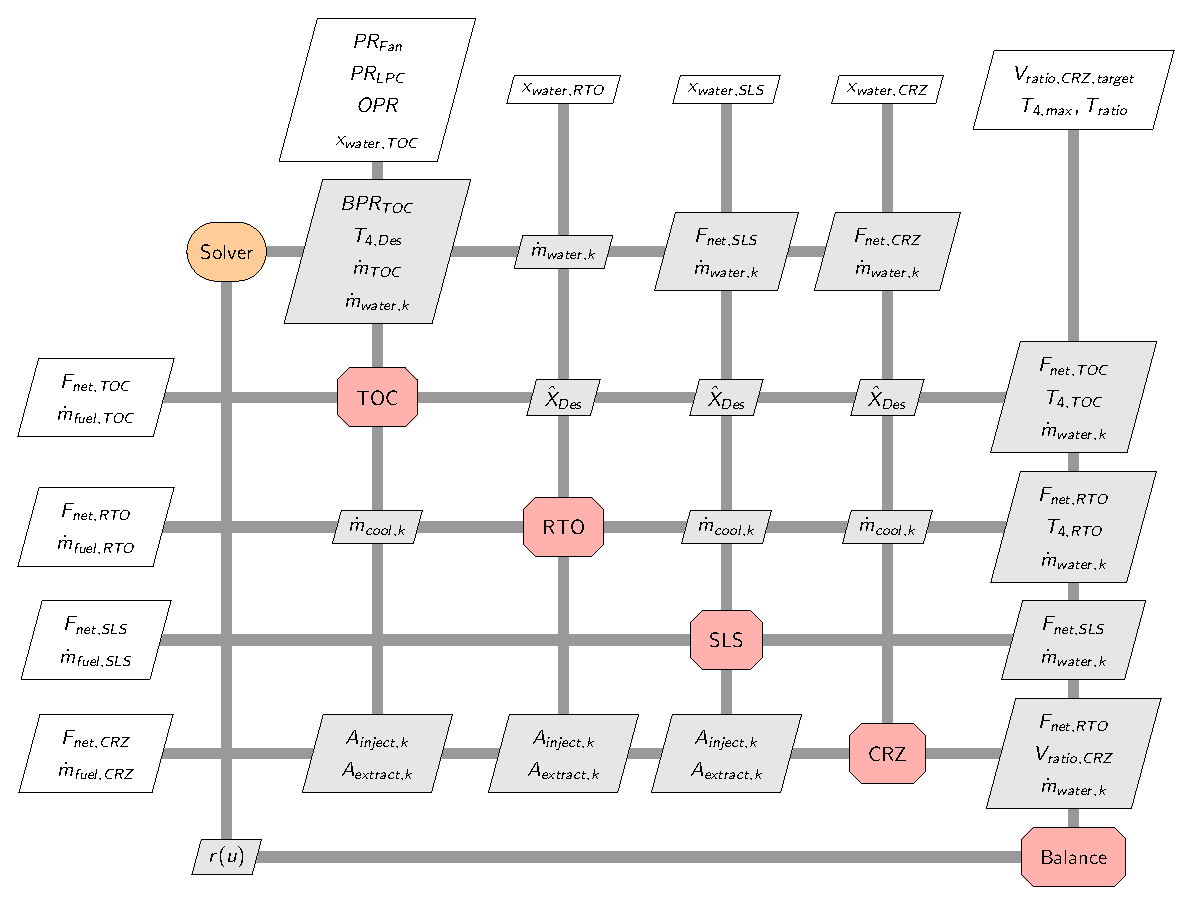
\includegraphics[width=\textwidth]{N3_xdsm_full.pdf}
  \caption{
    Full multidisciplinary design analysis (MDA) model N+3 XDSM diagram.
    This XDSM diagram shows the multipoint coupling between the different operation conditions and shows how the water recovery fractions are used to solve for water mass flow rates.
  }
  \label{fig:N3_xdsm_full}
\end{figure}

\section{Optimization Problem}
\label{sec:optprob}

We performed MDP gradient-based design optimization of the N+3 engine model considering the TOC, RTO, SLS, and CRZ flight conditions.
The objective is to minimize fuel burn subject to design and performance constraints.
Typical gas-turbine analysis measures the efficiency using the thrust-specific fuel consumption (TSFC).
However, this metric is not useful in the comparison of efficiency between Jet-A and hydrogen fueled cycle models because of the differences in fuel density and energy capacity.
A better metric for comparing Jet-A versus hydrogen is thrust-specific energy consumption (TSEC)~\cite{Adler2023}.
TSEC is TSFC multiplied by the lower heating value (LHV) of the fuel shown in Equation~\eqref{eq:tsec}.

\begin{equation}
  \mathrm{TSFC} = \frac{\dot{m}_{\mathrm{fuel}}}{F_{\mathrm{thrust}}}
  \label{eq:tsfc}
\end{equation}

\begin{equation}
  \mathrm{TSEC} = \frac{\dot{m}_{\mathrm{fuel}} \mathrm{LHV}}{F_{\mathrm{thrust}}} = \mathrm{TSFC} \times \mathrm{LHV}
  \label{eq:tsec}
\end{equation}

TSEC will be used as a efficiency metric at the cruise condition to compare the two fuels in the results.
The fuel properties used in the engine model are given in Table~\ref{fuel_props}~\footnote{\url{https://www.smartcockpit.com/docs/Jet_Fuel_Characteristics.pdf}}~\footnote{\url{https://www.engineeringtoolbox.com/fuels-higher-calorific-values-d_169.html}}.

\begin{table}[hbt!]
  \centering
  \caption{
    N+3 model fuel properties.
    The lower heating values are given for each fuel used to compute TSEC.}
  \begin{tabular}{r r r l}
    \hline
    Parameter              & Value & Units        & Description                  \\
    \hline
    $\rm{LHV}_{\rm{JetA}}$ & 18564 & \si{BTU/lbm} & Lower heating value of Jet-A \\
    $\rm{LHV}_{\rm{H2}}$   & 51591 & \si{BTU/lbm} & Lower heating value of H2    \\
    \hline
  \end{tabular}
  \label{fuel_props}
\end{table}

We present a high-level summary of the optimization framework using an XDSM diagram in Figure~\ref{fig:N3_opt_xdsm}.
The XDSM diagram shows the design variable, objective, and constraint connections between the optimization algorithm and the multipoint analysis model.
The detailed optimization problem description is provided in Table~\ref{tab:opt_problem}.

\begin{figure}[!hbt]
  \centering
  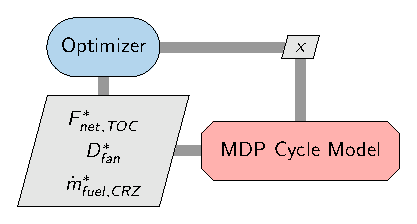
\includegraphics[width=0.5\textwidth]{N3_opt_XDSM.pdf}
  \caption{
    XDSM diagram of the multipoint optimization problem with objective, constraints, and MDA block.
    The XDSM diagram shows the variables and outputs within the optimization model and how each of these values is connected to the optimizer and MDA block.}
  \label{fig:N3_opt_xdsm}
\end{figure}

\begin{table}[hbt!]
  \centering
  \caption{
    Multipoint optimization problem definition.
    The objective function is the fuel flow rate at the cruise condition.
    The constraints are net thrust and engine diameter constraint at the design point, TOC.
  }
  \small
  \renewcommand{\arraystretch}{1.2}
  \begin{tabular}{r l l r l}
    \toprule
                    & Variable/Function              & Description                                                              & Units          & Quantity \\
    \hline
    minimize        & $\dot{m}_{\rm{fuel,CRZ}} $     & Fuel flow rate at CRZ                                                    & \si{lbm/s}     & 1        \\
                    &                                &                                                                          &                &          \\
    with respect to & $X_{\rm{H_2O,CRZ}}$            & Water recovery mass fraction at CRZ                                      & -              & 1        \\
                    & $\rm{PR}_{\rm{fan,TOC}}$       & TOC fan pressure ratio                                                   & -              & 1        \\
                    & $\rm{PR}_{\rm{LPC,TOC}}$       & TOC low-pressure compressor pressure ratio                               & -              & 1        \\
                    & $\rm{OPR}_{\rm{TOC}}$          & TOC overall pressure ratio                                               & -              & 1        \\
                    & $T_{4,\rm{RTO}}$               & RTO combustor temperature                                                & \si{\degree R} & 1        \\
                    & $T_{4,\rm{ratio}}$             & TOC-to-RTO temperature ratio (Equation~\eqref{t4ratio})                  & -              & 1        \\
                    & $V_{\rm{ratio,CRZ}}$           & Core-to-bypass nozzle velocity ratio at CRZ (Equation~\eqref{eq:vratio}) & -              & 1        \\
    \cline{3-5}
                    &                                & Total                                                                    &                & 7        \\
                    &                                &                                                                          &                &          \\
    subject to      & $F_{\rm{net,TOC}} \geq 5800.0$ & Target net thrust at TOC                                                 & \si{lbf}       & 1        \\
                    & $D_{\rm{fan}} \leq 100$        & Maximum Fan Diameter                                                     & \si{in^2}      & 1        \\
    \cline{3-5}
                    &                                & Total                                                                    &                & 2        \\
    \bottomrule
  \end{tabular}
  \label{tab:opt_problem}
\end{table}

The design variables are specified at different flight conditions.
At the TOC point, we include the fan pressure ratio ($\rm{PR}_{\rm{fan,TOC}}$), LPC pressure ratio ($\rm{PR}_{\rm{LPC,TOC}}$), and overall pressure ratio ($\rm{OPR}_{\rm{TOC}}$).
We add a design variable for maximum turbine inlet temperature at RTO ($T_{4,\rm{RTO}}$).
RTO is the limiting condition for the maximum allowable exit temperature of the burner.
The turbine inlet temperature at TOC is specified by a temperature ratio design variable ($T_{4,\rm{ratio}}$) between the RTO and TOC points, calculated as

\begin{equation}
  T_{4,\rm{ratio}} = \frac{T_{4,\rm{TOC}}}{T_{4,\rm{RTO}}}
  \label{t4ratio}
\end{equation}

\noindent
The nozzle velocity ratio at CRZ ($V_{\rm{ratio,CRZ}}$) is also added as a design variable to control the bypass ratio (BPR) at TOC.
The nozzle velocity ratio is defined as

\begin{equation}
  V_{\rm{ratio}} = \frac{V_{\rm{core,ideal}}C_{v,\rm{core}}}{V_{\rm{bypass,ideal}}C_{v,\rm{bypass}}}
  \label{eq:vratio}
\end{equation}
where $V_\text{ideal}$ is the ideal nozzle exit velocity and $C_v$ is the nozzle velocity coefficient that accounts for non-ideal nozzle effects.
The final design variable is the water recovery fraction at CRZ ($X_{\rm{H_2O,CRZ}}$).
We only include the water recovery fraction at cruise because it has the largest impact on the fuel mass flow rate objective function.
Additionally, the CRZ operating condition is the longest flight segment and contributes the most to long-term engine performance.
The range for each design variable and the associated units are shown in Table~\ref{tab:dv_table}.

\begin{table}[hbt!]
  \centering
  \caption{Design variable ranges for the optimization problem.
  }
  \small
  \renewcommand{\arraystretch}{1.2}
  \begin{tabular}{l l l l}
    Design Variable          & Lower  & Upper  & Units          \\
    \toprule
    $X_{\rm{H_2O,CRZ}}$      & 0.0    & 1.0    & -              \\
    $\rm{PR}_{\rm{fan,TOC}}$ & 1.2    & 1.4    & -              \\
    $\rm{PR}_{\rm{LPC,TOC}}$ & 2.5    & 4.0    & -              \\
    $\rm{OPR}_{\rm{TOC}}$    & 40.0   & 70.0   & -              \\
    $T_{4,\rm{ratio}}$       & 0.5    & 0.95   & -              \\
    $T_{4,\rm{RTO}}$         & 3000.0 & 3600.0 & \si{\degree R} \\
    $V_{\rm{ratio,CRZ}}$     & 1.35   & 1.45   & -              \\
    \bottomrule
  \end{tabular}
  \label{tab:dv_table}
\end{table}

As aforementioned in Section~\ref{sec:method}, the N+3 model uses balance relationships to enforce design, conservation, and performance requirements.
To create a reduced space optimization problem, the N+3 model imposes a set of constraints using additional balance relationships.
These constraints are satisfied using a Newton solver at the analysis level instead of the optimization level.
The advantage of the reduced space approach is that the design is feasible at the completion of each optimization iteration.
\citet{Martins2013} classify this architecture as multidisciplinary design feasible (MDF).
The balance relationships constrain the net thrust at the SLS and CRZ conditions, the BPR at TOC, and the turbine inlet temperature ($T_4$) at RTO.
We summarize the constraints as residuals (r) and the associated implicit states ($\vec{u}$) in Equation~\eqref{eq:balance_cons}.
\begin{equation}
  \label{eq:balance_cons}
  r(\vec{u}) \rightarrow
  \begin{cases}
    \setlength{\tabcolsep}{1pt}
    \begin{tabular}{l l}
      $r(\text{BPR}_\text{TOC})$    & $= (V_\text{ratio,TOC})_\text{des} - V_\text{ratio,TOC} = 0$, \\
      $r(\dot{m}_\text{total,TOC})$ & $= (T_{4,\text{RTO}})_\text{des} - T_{4,\text{RTO}} = 0$,     \\
      $r(\text{FAR}_\text{CRZ})$    & $= 0.9 F_\text{net, TOC} - F_\text{net, CRZ} = 0$,            \\
      $r(\text{FAR}_\text{SLS})$    & $= 1.2553 F_\text{net,RTO} - F_\text{net, SLS} = 0$.          \\
    \end{tabular}
  \end{cases}
\end{equation}

The N+3 pyCycle model is implemented in OpenMDAO~\cite{Gray2019a} to perform multidisciplinary gradient-based optimization with analytic coupled derivatives.
We use pyOptSparse~\cite{Wu2020a} to facilitate the use of state-of-the-art optimization software through a unified python interface.
We solve the optimization problem listed in Table~\ref{tab:opt_problem} with SNOPT~\cite{Gill2005a}, a gradient-based sequential quadratic programming (SQP) algorithm for large-scale constrained problems.
\section{Results}
\label{sec:results}

\subsection{Optimization Results}
\label{sub:opt_res}

We performed four optimizations of the N+3 engine cycle.
The optimizations considered Jet-A and hydrogen fuels with and without the water recovery loop.
For the optimizations without water recovery, we removed the water mass fraction design variable in Table~\ref{tab:opt_problem}.
In optimizations with water recovery, we use a constant $T_{4,\text{RTO}}$ from the optimizations without water recovery to aid comparisons between configurations.

The optimality and feasibility targets for the optimizations are both $10^{-6}$.
These optimizations took between 10--17 major SNOPT iterations to reach optimality and were completed in approximately 45 minutes on a standard laptop.
The optimality, feasibility, and merit function for each optimization is shown in Figure \ref{fig:history_summary}.
All four optimization problems converged to the requested feasibility and optimality tolerances.
The optimal design variables for each of the four optimizations are presented in Table~\ref{tab:dv_opt}.

% Feasibility, Optimality, Merit history
\begin{figure}[hbt!]
  \centering
  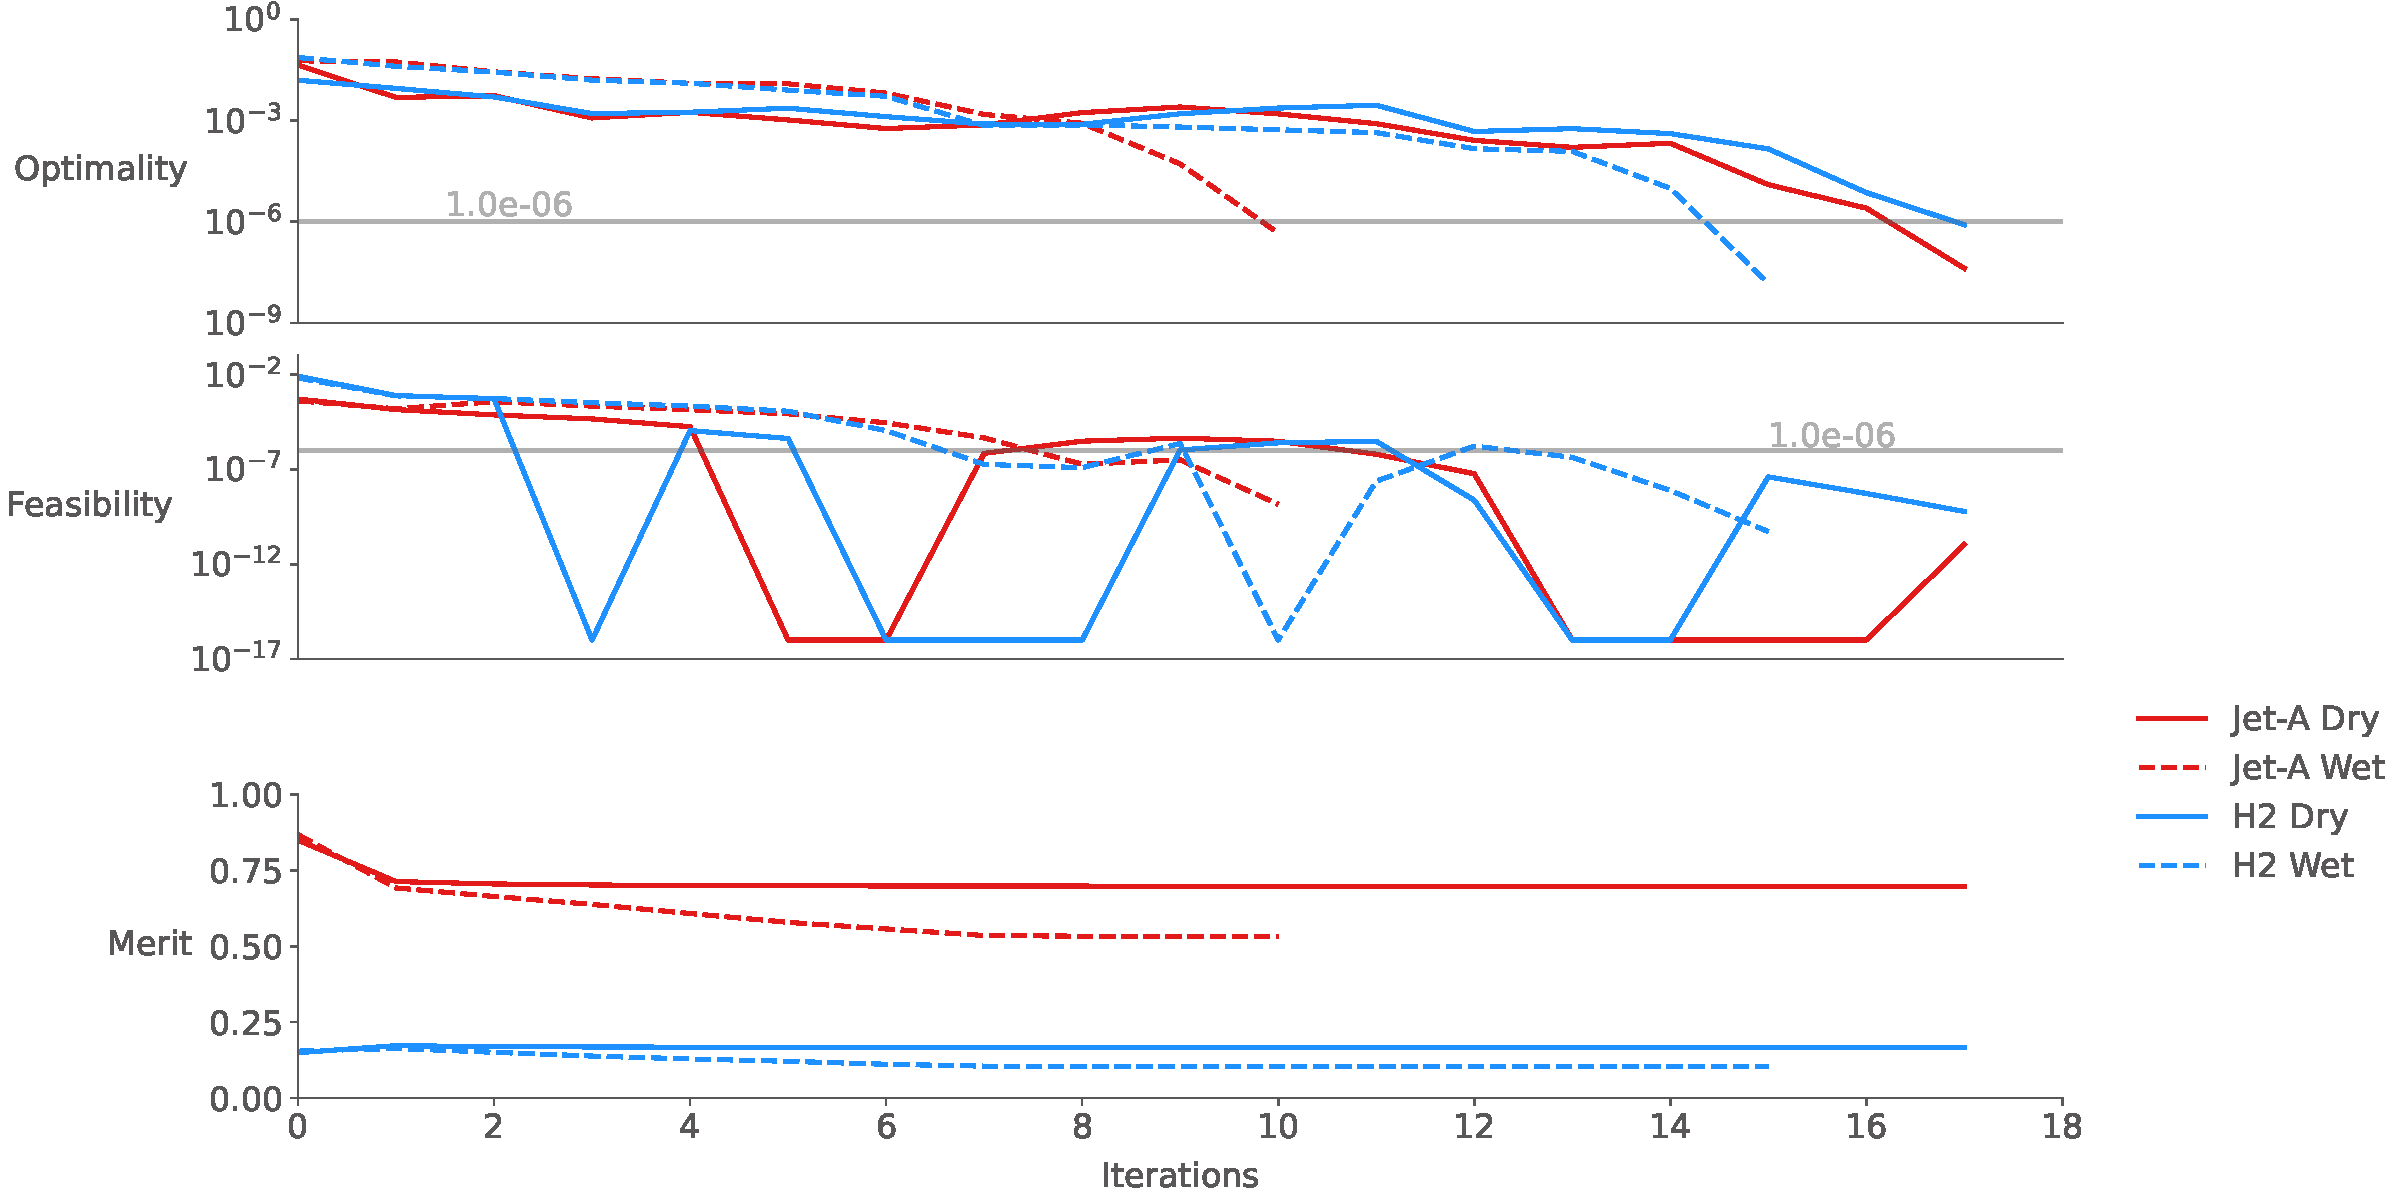
\includegraphics[width=1.0\textwidth]{opt_summary.pdf}
  \caption{The optimality, feasibility, and merit function history for each optimization problem.
    The red lines show Jet-A fuel and the blue lines show \ce{H2} fuel.
    The solid lines show the engine without water recovery and the dashed lines show the engine with water recovery.}
  \label{fig:history_summary}
\end{figure}

\begin{table}[hbt!]
  \centering
  \caption{Optimization results of the N+3 engine for four optimizations using Jet-A and hydrogen fuel with and without water recirculation.
  }
  \small
  \renewcommand{\arraystretch}{1.2}
  \begin{tabular}{r l l l l l l}
                & Variable/Function         & Jet-A Dry & Jet-A Wet & \ce{H2} Dry & \ce{H2} Wet & Units          \\
    \toprule
    objective   & $\dot{m}_{\rm{fuel,CRZ}}$ & 0.639     & 0.606     & 0.233       & 0.221       & \si{lbm/s}     \\
    % & $\rm{TSEC}_{\rm{CRZ}}$    & 8186.254  & 7766.338  & 8295.236    & 7859.635    & \si{lbm/hr/lbf} \\
    \hline
    variables   & $X_{\rm{H_2O,CRZ}}$       & -         & 0.3       & -           & 0.17        & -              \\
                & $\rm{PR}_{fan,TOC}$       & 1.285     & 1.292     & 1.288       & 1.297       & -              \\
                & $\rm{PR}_{LPC,TOC}$       & 4.0       & 4.0       & 4.0         & 4.0         & -              \\
                & $\rm{OPR}_{\rm{TOC}}$     & 61.012    & 61.188    & 60.660      & 61.952      & -              \\
                & $T_{4,\rm{ratio}}$        & 0.913     & 0.911     & 0.918       & 0.915       & -              \\
                & $T_{4,\rm{RTO}}$          & 3220.574  & -         & 3204.071    & -           & \si{\degree R} \\
                & $V_{\rm{ratio,CRZ}}$      & 1.35      & 1.35      & 1.35        & 1.35        & -              \\
    \hline
    constraints & $F_{\rm{net,TOC}}$        & 5800.0    & 5800.0    & 5800.0      & 5800.0      & \si{lbf}       \\
                & $D_{\rm{Fan}}$            & 100.0     & 100.0     & 100.0       & 100.0       & \si{in^2}      \\
    \bottomrule
  \end{tabular}
  \label{tab:dv_opt}
\end{table}

We summarize the optimal values of important thermodynamic variables on a parallel coordinate plot in Figure~\ref{fig:parallel_coords}.
This figure compares the optimal overall design of the N+3 cycle across the four optimization problems.
The TSEC of Jet-A is less than hydrogen with and without water recovery.
However, the TSEC of the optimal cycle with hydrogen combustion and water recovery is less than Jet-A combustion without water recovery.
This suggests that a hydrogen fueled N+3 UHB turbofan with water recovery can compete with the efficiency of a standard Jet-A fueled cycle.

With the addition of water recovery, the propulsive efficiency increases and leads to higher fan pressure ratios and lower TSEC for both fuels.
Additionally, the $T_{4,\text{ratio}}$ is reduced with water recovery leading to cooler combustion temperatures at TOC and subsequently lower fuel burn at CRZ.
We observe the optimal $T_{4,\text{RTO}}$ is larger for Jet-A than hydrogen because hydrogen has a larger combustion flammability limit and the engine can burn at a lower equivalence ratio to attain the same thrust requirements~\cite{Adler2023}.
Burning leaner lowers the FAR which reduces the fuel consumption for a given engine flow rate and is favorable for emissions reduction.
$V_\text{ratio,CRZ}$ is at the lower bound for all four cases to maximize the amount of mass flow through the bypass stream.

\begin{figure}[hbt!]
  \centering
  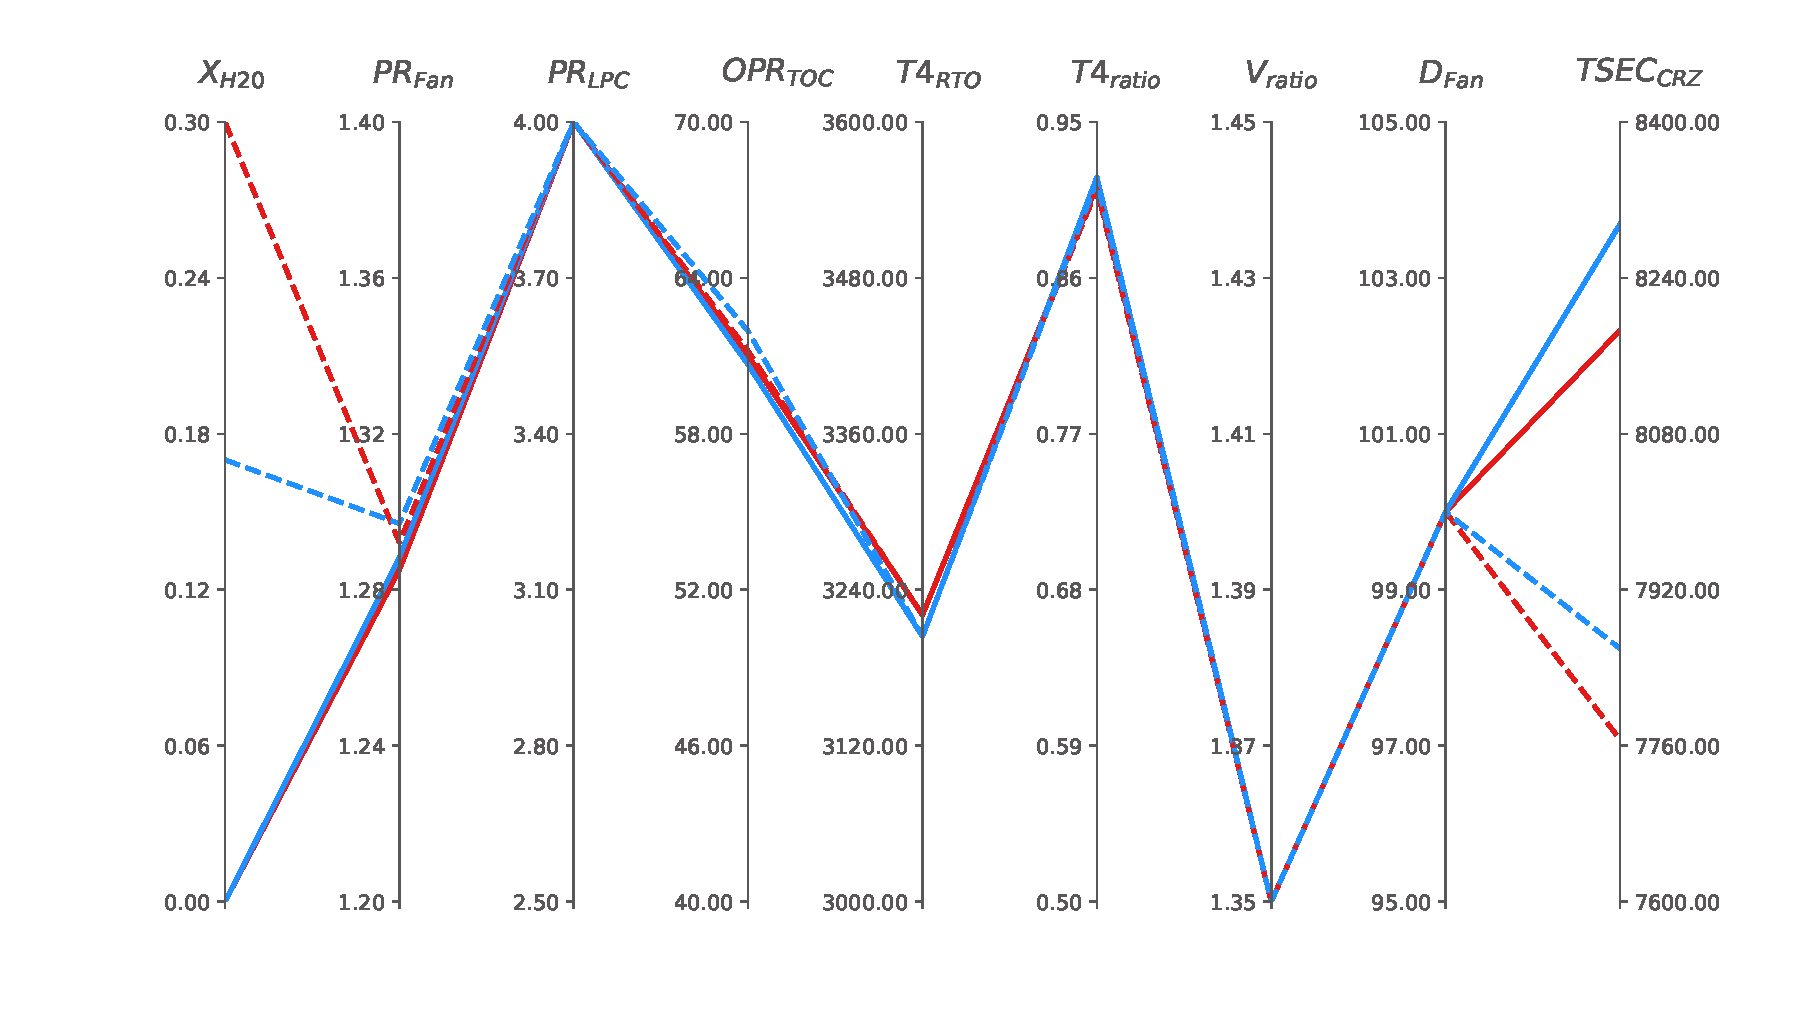
\includegraphics[width=1.0\textwidth]{N3_parallel_coords.pdf}
  \caption{Optimization results of the N+3 engine with and without water recovery using Jet-A and \ce{H2} as the fuel.
    The red lines show Jet-A fuel and the blue lines show \ce{H2} fuel.
    The solid lines show the engine without water recovery and the dashed lines show the engine with water recovery.}
  \label{fig:parallel_coords}
\end{figure}

\begin{figure}[hbt!]
  \centering
  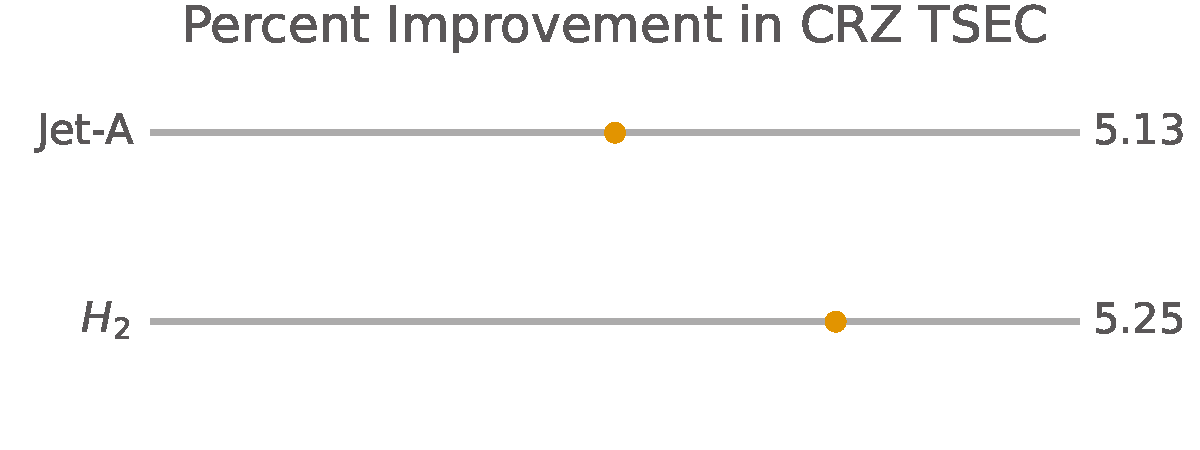
\includegraphics[width=0.65\textwidth]{bar_chart.pdf}
  \caption{Percent relative improvement in thrust specific energy consumption (TSEC) of the N+3 engine with water recovery.
    This plot compares the relative improvement of the two optimization problems with water recovery compared to the optimization problems without water recovery.
    The relative performance of hydrogen with water recovery compared to Jet-A without water recovery is also shown.}
  \label{fig:barchart}
\end{figure}

The TSEC improvement at CRZ due to water recovery for both fuels is shown on a bar chart in Figure~\ref{fig:barchart}.
Water recovery improves the TSEC approximately 5\% for both Jet-A and hydrogen fueled cycles.
Most of the design variables for the optimal designs with and without water recovery vary only slightly for both fuels.
This suggests that the water recovery system accounts for a majority of the efficiency improvements.
Achieving a 5\% reduction in TSEC represents a large fuel savings over the lifecycle of an engine.
As~\citeauthor{Strom2002} point out, a hydrogen-fueled engine would have close to 3 times more water in the exhaust than a similar Jet-A fueled counterpart.
The optimal designs with water recovery have approximately \SI{2.38}{lbm/s} and \SI{1.08}{lbm/s} of water in the core stream for hydrogen and Jet-A, respectively.
Hydrogen combustion offers an immediate reduction in emissions and produces more water in the exhaust stream.
With an advanced water recovery system, we can achieve better TSEC with hydrogen fuel than a standard Jet-A engine without water recovery.
To make hydrogen fueled engines a reality, we need to take advantage of the additional benefits of hydrogen combustion.
\subsection{Condenser Design Space Study}
\label{sub:dpqp_sweep}

The efficiency improvement due to water recirculation warrants a design space study for potential condenser technology.
Companies that are developing engines with water recirculation suggest that hydrogen can be used to as the heat sink for a water condenser~\cite{arpa-e_2021}.
We consider a condenser designed to fit inside the exhaust stream of a hydrogen-fueled turbofan engine.
The trade space for a condenser in the exhaust stream depends on the pressure loss and water recovery capability.

We model the pressure loss across the condenser by varying the relative total pressure loss across Duct5 just upstream of the core nozzle.
This pressure loss coefficient (dPqP) is the difference in total pressure across the duct divided by the total pressure at the duct inlet.
We varied the total pressure loss across the duct to simulate an increasingly larger condenser jutting out into the duct.
We ran an optimization to minimize fuel mass flow rate of hydrogen at each pressure loss value using the formulation for water recovery in Table~\ref{tab:opt_problem}.
The mass fraction of extracted water is held constant at 17\% to make a fair comparison at each pressure loss point.

\begin{figure}[hbt!]
  \centering
  \begin{subfigure}[t]{0.48\textwidth}
    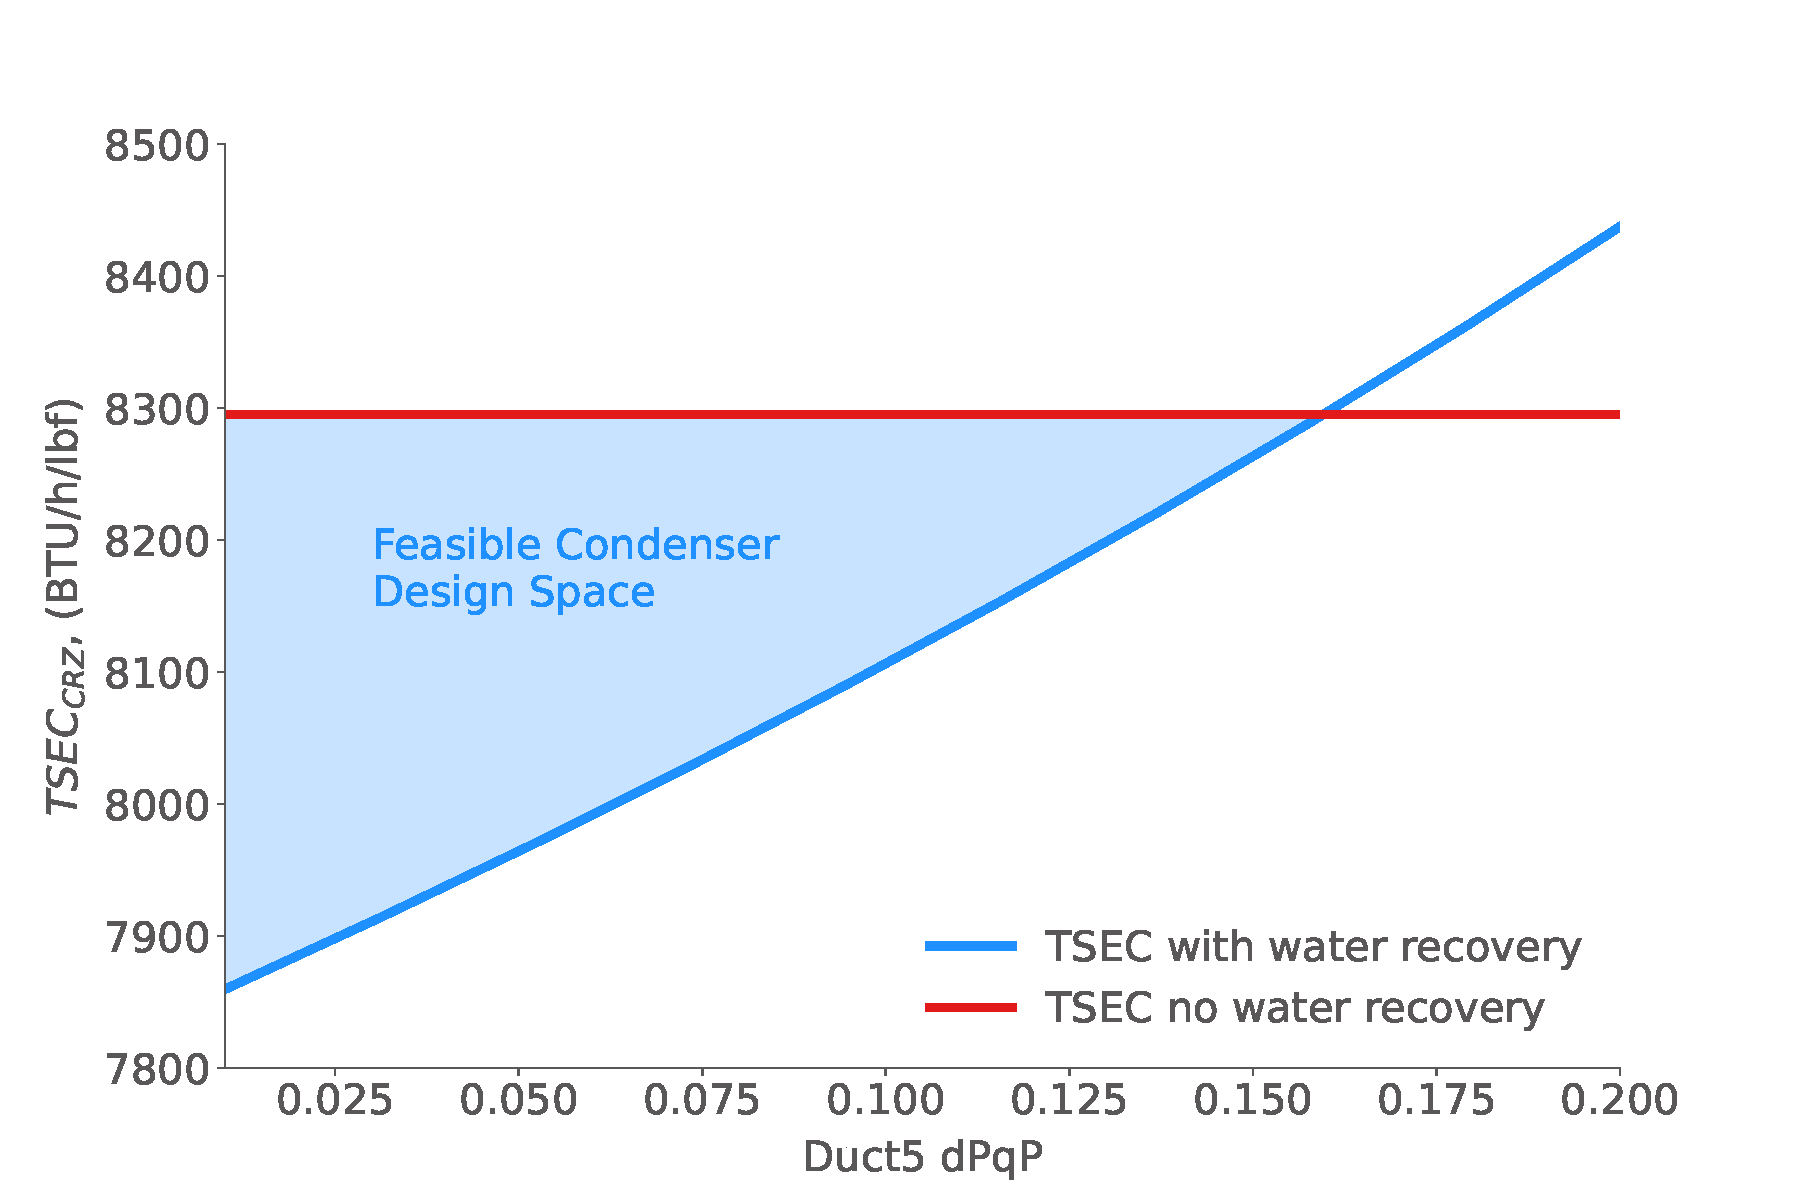
\includegraphics[width=\textwidth]{N3_dpqp.pdf}
    \caption{
      The figure shows the optimized TSEC values for varying levels of pressure loss due to the condensation of water compared to the optimization problem without water recovery.
      This shows the feasible space available for designing a water condenser while still benefiting from water recovery.}
    \label{fig:dpqp_sweep}
  \end{subfigure}
  \hspace{2pt}
  \begin{subfigure}[t]{0.48\textwidth}
    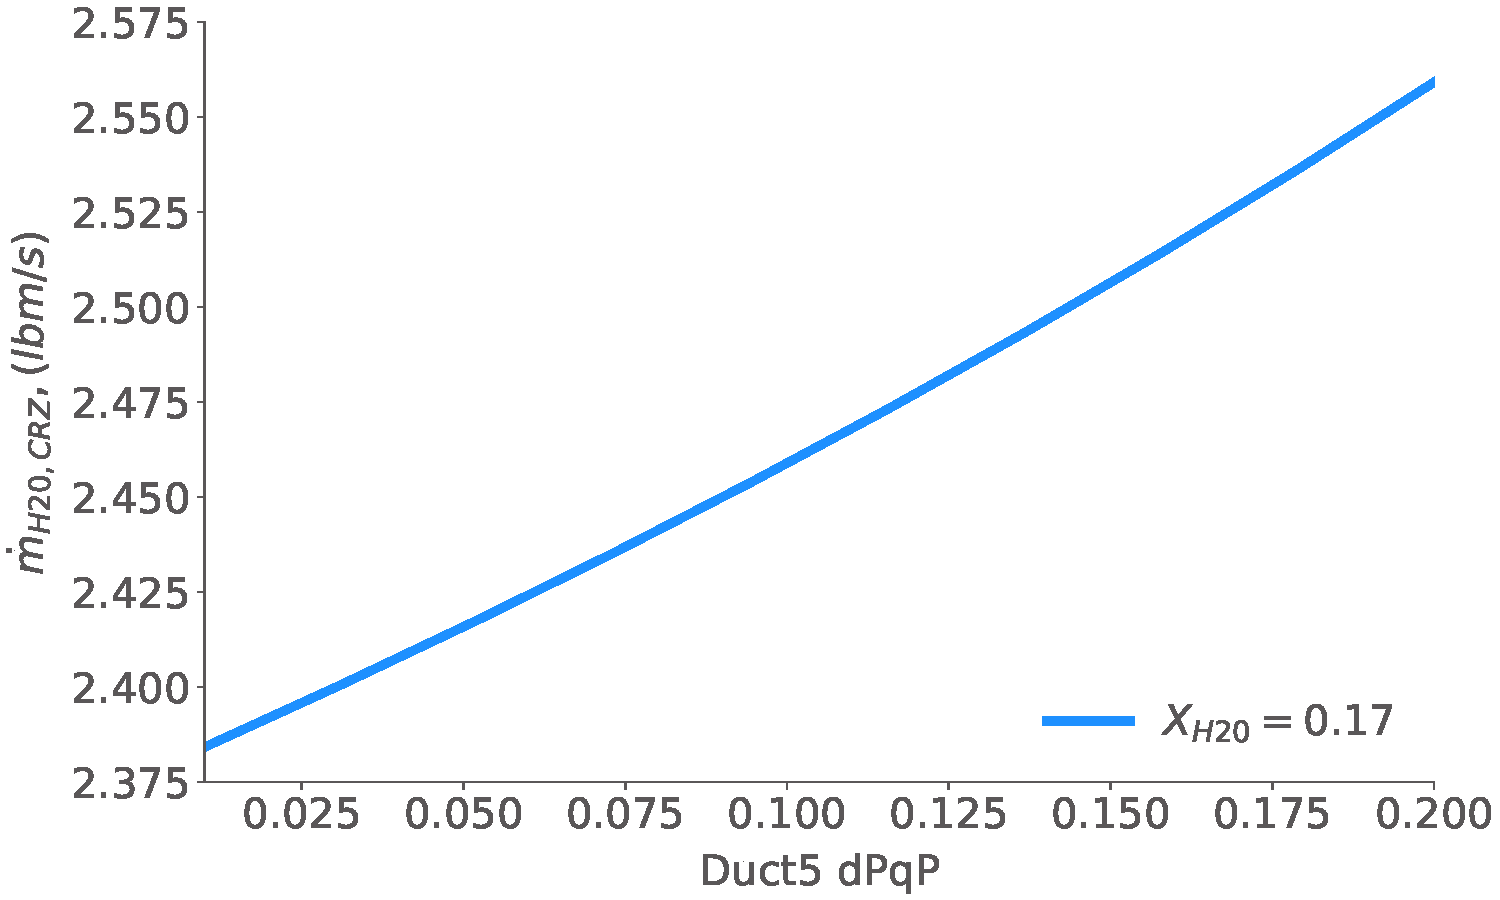
\includegraphics[width=\textwidth]{N3_wdot.pdf}
    \caption{
      The figure shows the optimal mass flow rate of water extracted at each pressure loss value.
    }
    \label{fig:dpqp_wdot}
  \end{subfigure}
  \caption{Pressure loss sweep of Duct5.
    Duct5 is just upstream of the water vapor extractor component.}
  \label{fig:dpqp_study}
\end{figure}

Figure~\ref{fig:dpqp_sweep} shows the $\rm{TSEC}_{\rm{CRZ}}$ of the optimal engine cycles plotted against dPqP.
The red horizontal line is the $\text{TSEC}_\text{CRZ}$ value of the optimized engine with no water recovery.
The blue region represents the feasible space for potential condenser technology.
The breakeven point where water recovery is no longer beneficial occurs at a pressure loss of roughly 0.16, or 16\%.
This estimate is based on an ideal condenser that can achieve the optimal water extraction for a given pressure loss.
In reality, losses due to inefficiencies further reduce the size of the feasible space.
The sensitivity of water extraction with respect to pressure loss is shown in Figure~\ref{fig:dpqp_wdot}.
The optimizer increases the amount of water extraction to compensate for the increasing pressure loss.
This represents a benchmark for designing condenser technology that can operate within the proposed water recirculation system.
The hydrogen fuel would serve a double purpose in this cycle.
The cold hydrogen fuel can be used as a heat sink for the condenser and then injected into the combustor at a higher temperature, further improving efficiency~\cite{Boggia2002}.

% Motivation: space to work with hydrogen, benefits of water injection, benefits of H2 (a lot of water, no tanks, de-mineralized water)
\section{Conclusion}
\label{sec:conc}
In this paper, we described a novel closed-loop water recirculation system for commercial aviation engines.
The water recirculation system was designed and implemented within the N+3 ultra-high bypass engine model.
We presented the results of four optimization problems demonstrating the use of this technology within a pyCycle model for Jet-A and hydrogen fuels.

The water recirculation system introduced two pyCycle components, namely the water extractor and injector, that form a continuous closed-loop feedback cycle in the engine.
We optimized the engine cycle considering Jet-A and hydrogen fuels with and without water recovery.
The objective was to minimize fuel mass flow rate subject to net thrust and fan diameter constraints.
The results show that optimal hydrogen-fueled engines with water recirculation are more efficient than standard Jet-A with no water recovery.
We demonstrated that the increased availability of water from hydrogen combustion proves the viability of this concept.
Additionally, hydrogen combustion eliminates carbon emissions and the lean fuel-to-air ratios result in cooler turbine inlet temperatures compared to Jet-A.

We performed a design space study to understand the technology requirements for a condenser that might operate in the proposed water recovery system.
The results showed that a hydrogen-fueled cycle with water recovery can sustain a pressure loss of 16\% across a condenser before the efficiency benefits diminish.
The thermal properties of hydrogen provide a heat sink and thus a readily available resource for water condensation within the condenser.
The hydrogen fuel absorbs heat and is then used in the combustion process, further improving engine efficiency.
Hydrogen-fueled UHBR turbofan engines can be more efficient than Jet-A counterparts when optimized considering water recovery.
Taking advantage of the beneficial properties of hydrogen is paramount for new engine technologies that can reduce emissions while improving performance.

\section{Acknowledgements}
\noindent
We would like to thank Justin Gray for his support in the development of the water recovery pyCycle models.

\bibliography{mdolab,references}

\end{document}